\documentclass[tikz,border=12pt]{standalone}
\usepackage{pgfplots}

\begin{document}
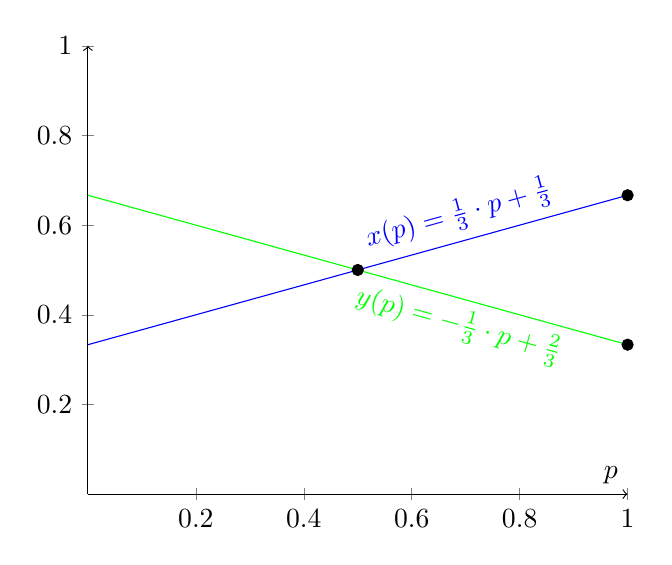
\begin{tikzpicture}
    \begin{axis}[
            xmin=0,xmax=1,
            ymin=0,ymax=1,
            axis x line=middle,
            axis y line=middle,
            axis line style=->,
            xlabel={$p$},
        ]
        \addplot [only marks] coordinates {(.5, .5) (1, 1/3) (1, 2/3)};
        \addplot[no marks,blue,-] expression[domain=0:1,samples=100]{1/3 * x + 1/3}
        node[above, sloped, pos = .7]{$x(p)=\frac{1}{3}\cdot p + \frac{1}{3}$};
        \addplot[no marks,green,-] expression[domain=0:1,samples=100]{-1/3 * x + 2/3}
        node[below, sloped, pos = .7]{$y(p)=-\frac{1}{3}\cdot p + \frac{2}{3}$};
    \end{axis}
\end{tikzpicture}
\end{document}
